%%% File-Information {{{
%%% Filename: template_bericht.tex
%%% Purpose: lab report, technical report, project report
%%% Time-stamp: <2004-06-22 23:36:32 xx>
%%% Authors: The LaTeX@TUG-Team [http://latex.tugraz.at/]:
%%%          Karl Voit (vk), Michael Prokop (mp), Stefan Sollerer (ss)
%%% History:
%%%   20040625 (vk,ss) initial version
%%%
%%% Notes:
%%%
%%%
%%%
%%% }}}
%%%%%%%%%%%%%%%%%%%%%%%%%%%%%%%%%%%%%%%%%%%%%%%%%%%%%%%%%%%%%%%%%%%%%%%%%%%%%%%%
%%% main document {{{

\documentclass[
a4paper,     %% defines the paper size: a4paper (default), a5paper, letterpaper, ...
% landscape,   %% sets the orientation to landscape
% twoside,     %% changes to a two-page-layout (alternatively: oneside)
% twocolumn,   %% changes to a two-column-layout
 headsepline, %% add a horizontal line below the column title
% footsepline, %% add a horizontal line above the page footer
% titlepage,   %% only the titlepage (using titlepage-environment) appears on the first page (alternatively: notitlepage)
 parskip=half,
% halfparskip,     %% insert an empty line between two paragraphs (alternatively: halfparskip, ...)
% leqno,       %% equation numbers left (instead of right)
 fleqn,       %% equation left-justified (instead of centered)
% tablecaptionabove, %% captions of tables are above the tables (alternatively: tablecaptionbelow)
% draft,       %% produce only a draft version (mark lines that need manual edition and don't show graphics)
% 10pt         %% set default font size to 10 point
% 11pt         %% set default font size to 11 point
12pt         %% set default font size to 12 point
]{scrartcl}  %% article, see KOMA documentation (scrguide.dvi)



%%%%%%%%%%%%%%%%%%%%%%%%%%%%%%%%%%%%%%%%%%%%%%%%%%%%%%%%%%%%%%%%%%%%%%%%%%%%%%%%
%%%
%%% packages
%%%

%%%
%%% encoding and language set
%%%
\usepackage[utf8]{inputenc}
\usepackage[T1]{fontenc}
\usepackage{ngerman} % which should have the same result as \usepackage[ngerman]{babel}
\usepackage{float}
%%%
%%% technical packages
%%%

%%% amsmath, amssymb, amstext: support for mathematics
\usepackage{amsmath,amssymb,amstext}

%%% psfrag: replace PostScript fonts
%\usepackage{psfrag}


%%% units: technical units
\usepackage{units}

%% listings: sourcecode
\usepackage{listings}

%% colors
\usepackage{color}

\definecolor{mygreen}{rgb}{0,0.6,0}
\definecolor{mygray}{rgb}{0.5,0.5,0.5}
\definecolor{mymauve}{rgb}{0.58,0,0.82}

%%%
%%% layout
%%%

%%% scrpage2: KOMA heading and footer
%%% Note: if you don't use this package, please remove 
%%%       \pagestyle{scrheadings} and corresponding settings
%%%       below too.
\usepackage{scrpage2}

%%%
%%% PDF
%%%

%%%\newif\ifpdf
%%%  \ifx\pdfoutput\undefined
%%%     \pdffalse
%%%  \else
%%%     \pdfoutput=1
%%%     \pdftrue
%%%  \fi

%%% Should be LAST usepackage-call!
%%% For docu on that, see reference on package ``hyperref''
\ifpdfoutput{%   (definitions for using pdflatex instead of latex)

  %%% graphicx: support for graphics
  \usepackage[pdftex]{graphicx}

  \pdfcompresslevel=9

  %%% hyperref (hyperlinks in PDF): for more options or more detailed
  %%%          explanations, see the documentation of the hyperref-package
  \usepackage[%
    %%% general options
    pdftex=true,      %% sets up hyperref for use with the pdftex program
    %plainpages=false, %% set it to false, if pdflatex complains: ``destination with same identifier already exists''
    %
    %%% extension options
    backref=true,      %% if true, adds a backlink text to the end of each item in the bibliography
    pagebackref=false, %% if true, creates backward references as a list of page numbers in the bibliography
    colorlinks=false,   %% turn on colored links (true is better for on-screen reading, false is better for printout versions)
    %
    %%% PDF-specific display options
    bookmarks=true,          %% if true, generate PDF bookmarks (requires two passes of pdflatex)
    bookmarksopen=false,     %% if true, show all PDF bookmarks expanded
    bookmarksnumbered=false, %% if true, add the section numbers to the bookmarks
    %pdfstartpage={1},        %% determines, on which page the PDF file is opened
    pdfpagemode=None         %% None, UseOutlines (=show bookmarks), UseThumbs (show thumbnails), FullScreen
  ]{hyperref}


  %%% provide all graphics (also) in this format, so you don't have
  %%% to add the file extensions to the \includegraphics-command
  %%% and/or you don't have to distinguish between generating
  %%% dvi/ps (through latex) and pdf (through pdflatex)
}{%else   (definitions for using latex instead of pdflatex)
  \usepackage[dvips]{graphicx}

  \usepackage[%
    dvips,           %% sets up hyperref for use with the dvips driver
    colorlinks=false %% better for printout version; almost every hyperref-extension is eliminated by using dvips
  ]{hyperref}

}


%%% sets the PDF-Informations options
%%% (see fields in Acrobat Reader: ``File -> Document properties -> Summary'')
%%% Note: this method is better than as options of the hyperref-package (options are expanded correctly)
\hypersetup{
  pdftitle={Routentracker für Schweizmobil}, %%
  pdfauthor={Schmid}, %%
  pdfsubject={}, %%
  pdfcreator={Accomplished with LaTeX2e and pdfLaTeX with hyperref-package.}, %% 
  pdfproducer={}, %%
  pdfkeywords={} %%
}


%%%%%%%%%%%%%%%%%%%%%%%%%%%%%%%%%%%%%%%%%%%%%%%%%%%%%%%%%%%%%%%%%%%%%%%%%%%%%%%%
%%%
%%% user defined commands
%%%

%%% \mygraphics{}{}{}
%% usage:   \mygraphics{width}{filename_without_extension}{caption}
%% example: \mygraphics{0.7\textwidth}{rolling_grandma}{This is my grandmother on inlinescates}
%% requires: package graphicx
%% provides: including centered pictures/graphics with a boldfaced caption below
%% 
\newcommand{\mygraphics}[3]{
  \begin{center}
    \includegraphics[width=#1, keepaspectratio=true]{#2} \\
    \textbf{#3}
  \end{center}
}

%%%%%%%%%%%%%%%%%%%%%%%%%%%%%%%%%%%%%%%%%%%%%%%%%%%%%%%%%%%%%%%%%%%%%%%%%%%%%%%
%%% Glossar
\usepackage{glossaries}

\makeglossaries

\newglossaryentry{population}
{
  name=Population,
  description={ist die Menge aller Individuen in einem evolutionären Algorithmus}
}
\newglossaryentry{individuum}
{
  name=Individuum,
  description={ist Teil der Population. Entspricht in unserem Falle einem endlichen Automaten oder einem endlichen Automaten mit Problemmenge}
}
\newglossaryentry{loesungskandidat}
{
  name=Lösungskandidat,
  description={wird als Synonym für Individuum verwendet}
}
\newglossaryentry{deepcopy}
{
  name={Deep Copy},
  description={Eine Kopie eines Objektes bei welchem auch alle enthaltenen Objekte kopiert wurden}
}
\newglossaryentry{c_g_alg}
{
  name={GK Algorithmus},
  description={Ein evolutionärer Algorithmus mit einer globalen, konstanten Problemmenge}
}
\newglossaryentry{e_g_alg}
{
  name={GM Algorithmus},
  description={Ein evolutionärer Algorithmus mit einer globalen, mutierenden Problemmenge}
}
\newglossaryentry{e_l_alg}
{
  name={LM Algorithmus},
  description={Ein evolutionärer Algorithmus mit lokalen, mutierenden Problemmengen}
}




%%%%%%%%%%%%%%%%%%%%%%%%%%%%%%%%%%%%%%%%%%%%%%%%%%%%%%%%%%%%%%%%%%%%%%%%%%%%%%%%
%%%
%%% define the titlepage
%%%

 \subject{Seminararbeit}   %% subject which appears above titlehead
% \titlehead{} %% special heading for the titlepage

%%% title
\title{Routentracker für Schweizmobil}

%%% author(s)
\author{Adrian Schmid}
\author{\texorpdfstring{Adrian Schmid - \href{mailto:schmiad1@students.zhaw.ch}{schmiad1@students.zhaw.ch}}{Adrian Schmid}}

%%% date
\date{Zürich, 04.06.2014}

% \publishers{}

% \thanks{} %% use it instead of footnotes (only on titlepage)

% \dedication{} %% generates a dedication-page after titlepage


%%% uncomment following lines, if you want to:
%%% reuse the maketitle-entries for hyperref-setup
%\newcommand\org@maketitle{}
%\let\org@maketitle\maketitle
%\def\maketitle{%
%  \hypersetup{
%    pdftitle={\@title},
%    pdfauthor={\@author}
%    pdfsubject={\@subject}
%  }%
%  \org@maketitle
%}


%%%%%%%%%%%%%%%%%%%%%%%%%%%%%%%%%%%%%%%%%%%%%%%%%%%%%%%%%%%%%%%%%%%%%%%%%%%%%%%%
%%%
%%% set heading and footer
%%%

%%% scrheadings default: 
%%%      footer - middle: page number
\pagestyle{scrheadings}

%%% user specific
%%% usage:
%%% \position[heading/footer for the titlepage]{heading/footer for the rest of the document}

%%% heading - left
% \ihead[]{}

%%% heading - center
% \chead[]{}

%%% heading - right
 \ohead[]{Routentracker für Schweizmobil}

%%% footer - left
% \ifoot[]{}

%%% footer - center
% \cfoot[]{}

%%% footer - right
% \ofoot[]{}



%%%%%%%%%%%%%%%%%%%%%%%%%%%%%%%%%%%%%%%%%%%%%%%%%%%%%%%%%%%%%%%%%%%%%%%%%%%%%%%%
%%%
%%% begin document
%%%

\setcounter{tocdepth}{2}


\begin{document}

  \lstset{ %
    backgroundcolor=\color{white},   % choose the background color; you must add \usepackage{color} or \usepackage{xcolor}
    basicstyle=\footnotesize,        % the size of the fonts that are used for the code
    breakatwhitespace=false,         % sets if automatic breaks should only happen at whitespace
    breaklines=true,                 % sets automatic line breaking
    captionpos=b,                    % sets the caption-position to bottom
    commentstyle=\color{mygreen},    % comment style
    deletekeywords={...},            % if you want to delete keywords from the given language
    escapeinside={\%*}{*)},          % if you want to add LaTeX within your code
    extendedchars=true,              % lets you use non-ASCII characters; for 8-bits encodings only, does not work with UTF-8
    frame=single,                    % adds a frame around the code
    keepspaces=true,                 % keeps spaces in text, useful for keeping indentation of code (possibly needs columns=flexible)
    keywordstyle=\color{blue},       % keyword style
    language=Octave,                 % the language of the code
    morekeywords={*,...},            % if you want to add more keywords to the set
    numbers=left,                    % where to put the line-numbers; possible values are (none, left, right)
    numbersep=5pt,                   % how far the line-numbers are from the code
    numberstyle=\tiny\color{mygray}, % the style that is used for the line-numbers
    rulecolor=\color{black},         % if not set, the frame-color may be changed on line-breaks within not-black text (e.g. comments (green here))
    showspaces=false,                % show spaces everywhere adding particular underscores; it overrides 'showstringspaces'
    showstringspaces=false,          % underline spaces within strings only
    showtabs=false,                  % show tabs within strings adding particular underscores
    stepnumber=1,                    % the step between two line-numbers. If it's 1, each line will be numbered
    stringstyle=\color{mymauve},     % string literal style
    tabsize=2,                       % sets default tabsize to 2 spaces
  }



 \pagenumbering{roman} %% small roman page numbers

%%% include the title
% \thispagestyle{empty}  %% no header/footer (only) on this page
 \maketitle

%\input{content/00_preface/abstract.tex}

\clearpage
%%% start a new page and display the table of contents
% \newpage
\tableofcontents
%%% display the main document on a new page 
% \newpage

 \pagenumbering{arabic} %% normal page numbers (include it, if roman was used above)

%%%%%%%%%%%%%%%%%%%%%%%%%%%%%%%%%%%%%%%%%%%%%%%%%%%%%%%%%%%%%%%%%%%%%%%%%%%%%%%%
%%%
%%% begin main document
%%% structure: \section \subsection \subsubsection \paragraph \subparagraph
%%%

\clearpage
\section{Einleitung}
\subsection{Ausgangslage}
Als begeisterter Velofahrer habe ich vor einiger Zeit die Tools (Website \& Smartphone App) der Stiftung Schweizmobil für mich entdeckt. Diese Platform bietet den Benutzern offizielle Swisstopo Karten auf welchen alle offiziellen Velo-, Mountainbike-, Wander-, Inlineskate- und Kanurouten eingeblendet werden können. Zusätzlich kann man als registrierter Benutzer auf der Website eigene Routen zeichnen. So gezeichnete Routen können ausgedruckt, geteilt oder auf die Schweizmobil App übertragen werden. Was die Tools nicht bieten ist eine \flqq Where have I been\frqq-Tracker Funktion um gefahrene Routen direkt aufzuzeichnen.

Ich habe die Stiftung Schweizmobil bezüglich des geplanten Projekts und einer Schnittstelle zum automatischen Übermitteln von GPS Daten angefragt. Aktuell gibt es die Möglichkeit Tracks aus Files im GPX Format als Routen zu importieren. Schweizmobil habe bei der Implementierung seiner App einen \flqq Where have I been\frqq-Tracker angedacht jedoch aufgrund Zweifel bezüglich Genauigkeit und Batterielebensdauer wieder verworfen. Sie seien an den Ergebnissen meiner potentiellen Arbeit interessiert.

\subsection{Ziele der Arbeit}
Im dieser Arbeit geht es in einem ersten Schritt um das erstellen eines sehr technischen \flqq Where have I been\frqq-Trackers welcher unter anderem einen Export von gefahrenen Routen ins GPX Format beherrscht. Mit diesem Tracker werden dann in einem zweiten Schritt Experimente durchgeführt um eine möglichst hohe Genauigkeit bei möglichst geringem Akkuverbrauch zu erreichen.

\subsection{Aufgabenstellung}
\begin{itemize}
\item Einarbeitung in das Thema GPS, GPS Tracking, GPX Format und Dokumentation des Erarbeiteten
\item Implementierung eines technischen \flqq Where have I been\frqq-Trackers zu versuchszwecken
\item Implementierung des Datenexports ins GPX Format
\item Durchführen verschiedener Tests bezüglich Akkuverbrauch und Genauigkeit
\item Präsentation der Arbeit
\end{itemize}

\subsection{Erwartete Resultate}
\begin{itemize}
\item Dokumentation der Einführung (GPS, GPS Tracking, GPX Format)
\item Implementation des \flqq Where have I been\frqq-Trackers inklusive Dokumentation
\item Implementation des GPX Datenexports inklusive Dokumentation
\item Dokumentation der Tests und Auswertung der Resultate
\item Präsentation
\end{itemize}
\clearpage
\section{Grundlagen}
\subsection{Grundlagen der Erdvermessung}
Um Karten oder Modelle der Erde zu erstellen, braucht es ein Vermessungssystem welches adäquat die Grösse und Form der Erde widerspiegelt. Wichtig beim Arbeiten mit einem solchen Modell ist, dass man sich bewusst ist, welche Annahmen getroffen wurden und welche Abweichungen aus sowohl der Messmethode als auch dem Modell entstehen. In diesem Kapitel geht es um die Klärung der Grundlagen die zum Verständnis der Funktionsweise des GPS notwendig sind. \cite{geodesy}

\begin{figure}[h]
  \centering
  \includegraphics[width=0.8\textwidth]{images/geoid.jpg}
  \caption[Erde, Geoid und Referenzellipsoid]{Verhältnis zwischen der Erdoberfläche, dem Geoiden und einem Referenzellipsoiden. \cite{geodesy}}
  \label{fig:geoid}
\end{figure}

Die Wissenschaft der Erdvermessung - auch Geodäsie - beschäftigt sich mit dem Studium von Grösse und Form der Erde, des Erdgravitationsfeldes und den Veränderungen des eben genannten. Zu den Grundlagen der Geodäsie gehört die Unterscheidung zwischen der physikalischen Erde, dem Geoid und dem Referenzellipsoid. Die physikalische Erde ist die Erde an sich. Der Geoid hat die Form, welche eine von Ozeanen bedeckte Erde, nur unter Einfluss von Gravitation und Rotation annehmen würde. Der Referenzellipsoid ist eine einfache, mathematische Form welche dem Geoid so gut als möglich entspricht. \cite{geodesy}

\subsection{Georeferenzierung}
Die Fähigkeit geografische Positionen genau zu beschreiben ist essentiell für sowohl Karten als auch geografische Informationssysteme. Diesen Prozess nennt man Georeferenzierung.

Eine geografische Position mithilfe von Längen- und Breitengraden auf dem Referenzellipsoiden zu beschreiben ist eine Möglichkeit der Georeferenzierung. Weitere Möglichkeiten wäre zum Beispiel die Verwendung von planaren oder kartesischen Koordinatensystemen. Im Umgang mit GPS werden ausschliesslich Längen- und Breitengrade verwendet, weshalb die weiteren Möglichkeiten im Rahmen dieser Arbeit nicht weiter erläutert werden.

Die Längen- und Breitengrade sind Winkelmessungen wischen dem Zentrum des entsprechenden Ellipsoiden und einem Punkt auf der Oberfläche. Breitengrade (in Englisch latitude) messen dabei den Winkel in Nord-Süd Richtung, Längengrade (in Englisch longitude) den Ost-West Winkel. \cite{georef}

\begin{figure}[h]
  \centering
  \includegraphics[width=0.5\textwidth]{images/longlat.png}
  \caption[Längen- und Breitengrade]{Lesen von Längen- und Breitengraden \cite{georef}}
  \label{fig:longlat}
\end{figure}

\subsection{World Geodetic System 1984}
Das World Geodetic System 1984 ist das geodätische Referenzsystem welches für GPS Positionsangaben verwendet wird. Als Koordinatenursprung dieses Systems dient das Massenzentrum der Erde. 

Dieses System besteht aus:
\begin{itemize}
	\item einem Referenzellipsoid für Ortsangaben nach geographischer Länge und Breite
	\item einem Geoid
	\item einem Satz dreidimensionaler Koordinaten der zwölf über die Erde verteilten Fundamentalstationen für die Verankerung der zuvor genannten Modelle in der Erdkruste \cite{wsg84}
\end{itemize}

\subsection{Global Positioning System}
TODO: Grobe Zusammenfassung der Funktionsweise von GPS. Ggf auf Basis von \cite{leicagps}

\subsection{Distanzberechnung zwischen GPS Koordinaten}
Zur Berechnung der Distanz zwischen zwei GPS Koordinaten wurde in dieser Arbeit die Haversine Formel verwendet: \cite{haversine} 

Definitionen:\\
\begin{equation}
\begin{array}{lcl}
\varphi_1, \varphi_2 & = & \text{Breitengrade}\\
\lambda_1, \lambda_2 & = & \text{Längengrade}\\
\Delta\varphi & = & \text{Differenz zwischen den Breitengraden}\\
\Delta\lambda & = & \text{Differenz zwischen den Längengraden}\\
R & = & \text{Radius der Erde}\\
\end{array}
\end{equation}

Berechnung:\\
\begin{equation}
\begin{array}{lcl}
a & = &\sin^2(\frac{\Delta\varphi}{2})+\cos \varphi_1 \cdot \cos \varphi_2 \cdot \sin^2(\frac{\Delta\lambda}{2})\\
c & = & 2 \cdot atan2(\sqrt{a}, \sqrt{(1-a)})\\
d & = & R \cdot c
\end{array}
\end{equation}

Diese Formel verwendet anstelle des Ellipsoiden eine Sphäre was bei grossen Distanzen zu Fehlern führen kann. Bei den Distanzen zwischen Messpunkten von Velotouren oder Wanderungen ist dieser Fehler nicht signifikant. Die Vorteile dieser Formel liegen in der einfachen Implementierbarkeit und der guten Performanz dieser Implementationen. 

\subsection{Das GPX Datenformat}
Das GPX oder GPS Exchange Format ist ein XML Schema zur Darstellung von GPS Daten. Es kann verwendet werden um \flqq Waypoints\frqq, \flqq Tracks\frqq und \flqq Routes\frqq darzustellen. Eine Ansammlung von \flqq Waypoints\frqq kann verwendet werden um eine Menge von Punkten darzustellen die in keinem sequenziellen Zusammenhang zueinander stehen. \flqq Routes\frqq und \flqq Tracks\frqq beinhalten sequenziell angeordnete \flqq Waypoints\frqq. Der Unterschied zwischen den Beiden ist, dass bei einer \flqq route\frqq nur Wegpunkte bei Richtungsänderungen abgebildet sind, den Rest muss sich das System daraus berechnen. Ein \flqq Track\frqq beinhaltet alle aufgezeichneten Punkte. Im Rahmen dieses Projektes werden \flqq Tracks\frqq aufgezeichnet. \cite{gpxwiki} \cite{gpx}

\begin{lstlisting}[language=XML, caption={GPX Beispielfile}]
<?xml version="1.0" encoding="UTF-8" standalone="no" ?>

<gpx xmlns="http://www.topografix.com/GPX/1/1" xmlns:gpxx="http://www.garmin.com/xmlschemas/GpxExtensions/v3" xmlns:gpxtpx="http://www.garmin.com/xmlschemas/TrackPointExtension/v1" creator="Oregon 400t" version="1.1" xmlns:xsi="http://www.w3.org/2001/XMLSchema-instance" xsi:schemaLocation="http://www.topografix.com/GPX/1/1 http://www.topografix.com/GPX/1/1/gpx.xsd http://www.garmin.com/xmlschemas/GpxExtensions/v3 http://www.garmin.com/xmlschemas/GpxExtensionsv3.xsd http://www.garmin.com/xmlschemas/TrackPointExtension/v1 http://www.garmin.com/xmlschemas/TrackPointExtensionv1.xsd">
  <metadata>
    <link href="http://www.garmin.com">
      <text>Garmin International</text>
    </link>
    <time>2009-10-17T22:58:43Z</time>
  </metadata>
  <trk>
    <name>Example GPX Document</name>
    <trkseg>
      <trkpt lat="47.644548" lon="-122.326897">
        <ele>4.46</ele>
        <time>2009-10-17T18:37:26Z</time>
      </trkpt>
    </trkseg>
  </trk>
</gpx>
\end{lstlisting}
\clearpage
\section{Umsetzung}
\subsection{Benutzerführung}
Die Applikation wurde so als Konsolenapplikation angelegt, dass alle Module auch einzeln verwendet werden können. Für Enduser wurde jedoch im \lstinline$starter.py$ ein Konsolen-gesteuerter Workflow implementiert.

\begin{enumerate}
	\item Titel für die Suche muss eingegeben werden
	\item Der Benutzer wird gefragt, ob er bereits vorhandene Twitterdaten analysieren will oder ob er neue Twitterdaten über das API herunterladen möchte.
	\begin{enumerate}
		\item Wenn der Benutzer neue Twitterdaten laden möchte wird er nach Schlüsselwörtern gefragt
		\item Dem Benutzer werden die eingegebenen Schlüsselwörter nochmals angezeigt und er muss bestätigen damit das API angestossen wird
		\item Die Daten werden heruntergeladen und im File \lstinline$keyword1_keyword2_...keywordn_raw_search_timestamp.txt$ abgelegt. Der Filepfad wird zurückgegeben.
	\end{enumerate}
	\item Wenn der Benutzer vorhandene Twitterdaten analysieren möchte, muss er den Pfad zum Twitterdatenfile angeben
	\item Der Benutzer bestätigt, dass er die Twitter Datenanalyse für die gegebenen Tweets starten möchte
	\item Das Programm analysiert die Daten, erstellt die Plots und ein Logfile mit Resultaten
\end{enumerate}

Live sieht dies wie in Abbildung \ref{fig:benutzerfuehrung} aus.

\begin{figure}[h]
  \centering
  \includegraphics[width=0.8\textwidth]{images/benutzerfuehrung.png}
  \caption[Benutzerführung]{Benutzerführung}
  \label{fig:benutzerfuehrung}
\end{figure}

\subsubsection{Verwendete bzw. Eingebundene Ressourcen}
\begin{table}[H]
\begin{center}
\begin{tabular}{|l|l|}
	\hline
	\lstlisting$starter.py$ & Enthält den Code der Benutzerführung \\ \hline
	\lstlisting$gather_twitterdata.py$ & Enthält die Methoden zum herunterladen der Tweets \\ \hline
	\lstlisting$analyse_twitterdata.py$ & Wird mit MPI angestossen um die Daten zu analysieren \\ \hline
\end{tabular}
\caption{Verwendete Ressourcen: Benutzerführung}
\end{center}
\end{table}


\subsection{Twitterdaten Sammeln}
Wie bereits im Kapitel \ref{subsec:grundlagentwitter} beschrieben wurde zum Herunterladen der Tweets das Package TwitterSearch von Christian Koepp\cite{twittersearch} verwendet. 


\subsection{Algorithmen zur Erkennung der Gefühlslage in Texten}
\subsubsection{Emoticons}
\subsubsection{SentiWordNet}
\subsubsection{SenticNet}
\subsubsection{SASA}
\subsubsection{NLTK naive Bayes}
\subsection{Parallelisierung}
\clearpage
\section{Analyse}
\subsection{Vergleich der Algorithmen}
Bei den Experimenten mit den verschiedenen Algorithmen ist aufgefallen, dass der Emoticon Algorithmus aufgrund der seltenen Verwendung von Emoticons in Tweets praktisch nicht funktioniert. Je ernster das Thema desto weniger Emoticons werden tendenziell verwendet. Folgend die Resultate zweier Twitter Downloads. Die Keywörter für den ersten Download waren \flqq switzerland \frqq und \flqq ecuador\frqq. Die Schweiz hat kurz zuvor am WM Auftaktspiel in der 93. Minute das entscheidende 2:1 gegen Ecuador geschossen. Die Keywörter für den zweiten Download waren \flqq ISIS\frqq und \flqq Iraq\flqq. ISIS ist eine militante Jihadistengruppe, die derzeit für unruhen im Nordiran sorgt. \cite{isis} Folgend werden diese Resultate beschrieben und es werden Thesen zu den Resultaten der Twitteranalysen aufgestellt. Um diese zu verifizieren oder zu falsifizieren, bräuchte man gelabelte Twitterdaten, welche im Rahmen dieser Arbeit nicht erarbeitet werden konnten.

\begin{figure}[h]
  \centering
  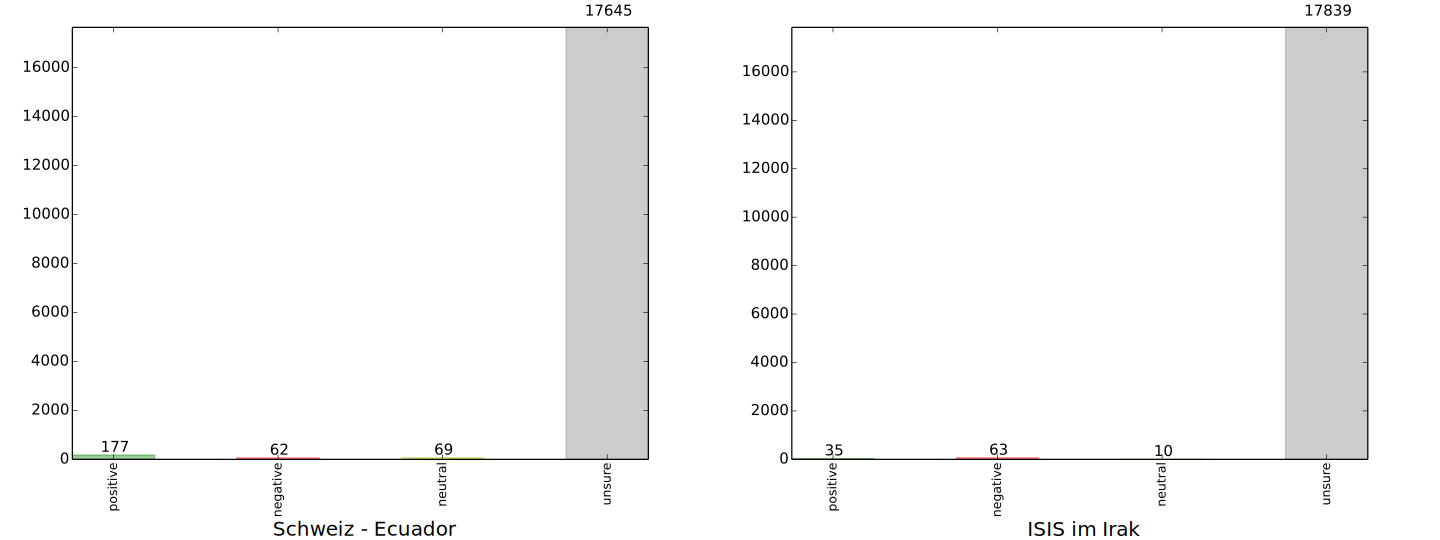
\includegraphics[width=0.8\textwidth]{images/schweizvsirak_emoticon.pdf}
  \caption[Emoticon Analyse: Schweiz - Ecuador vs. ISIS im Irak]{Emoticon Analyse: Schweiz - Ecuador vs. ISIS im Irak}
  \label{fig:emoticonanalysis}
\end{figure}

Die Resultate der in Abbildung \ref{fig:emoticonanalysis} sichtbaren Suche decken sich mit den Erkenntnissen aus vorhergehenden Suchläufen. In rund 1.7\% der Schweiz-Ecuador Tweets wurden Emoticons verwendet. Erfreulicherweise waren diese mehrheitlich positiv. Die Irak Tweets hatten lediglich einen Emoticon-Anteil von 0.6\% und diese waren meist negativ.

Beim der Twitteranalyse mithilfe des naiven Bayes der NLTK Library (Abbildung \ref{fig:naivebayesanalysis}) ist ersichtlich, wie sich die Wahl des Trainingsets auf das Ergebnis auswirkt. Movie Reviews (das hier verwendete Trainingset) sind üblicherweise längere Texte die, wenn positiv, sehr sachlich geschrieben sind. Beim manuellen durchsehen der Tweets fiel auf, dass viele Tweets zu ISIS im Irak Zeitungsüberschriften entsprechen oder einfach sehr sachlich geschrieben sind. Dies wird von diesem Klassifizierungsverfahren als positiv gewertet.

\begin{figure}[H]
  \centering
  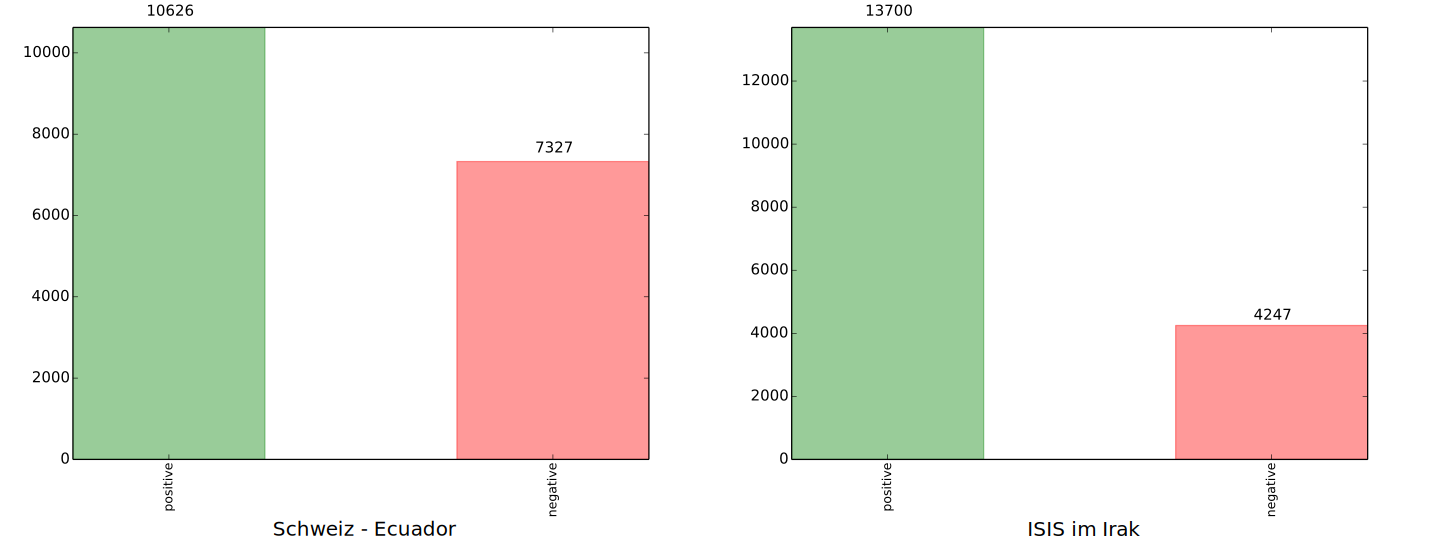
\includegraphics[width=0.8\textwidth]{images/schweizvsirak_nltk.pdf}
  \caption[NLTK Naive Bayes: Schweiz - Ecuador vs. ISIS im Irak]{NLTK Naive Bayes: Schweiz - Ecuador vs. ISIS im Irak}
  \label{fig:naivebayesanalysis}
\end{figure}

\begin{figure}[H]
  \centering
  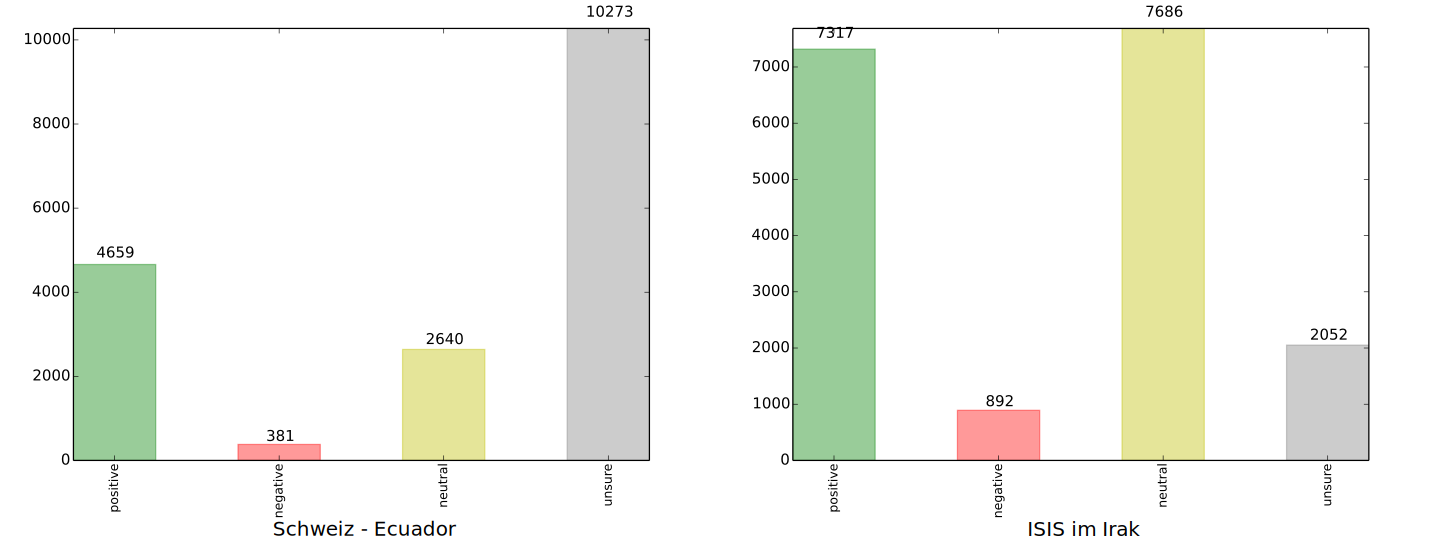
\includegraphics[width=0.8\textwidth]{images/schweizvsirak_sasa.pdf}
  \caption[SASA: Schweiz - Ecuador vs. ISIS im Irak]{SASA: Schweiz - Ecuador vs. ISIS im Irak}
  \label{fig:sasaanalysis}
\end{figure}

\begin{figure}[H]
  \centering
  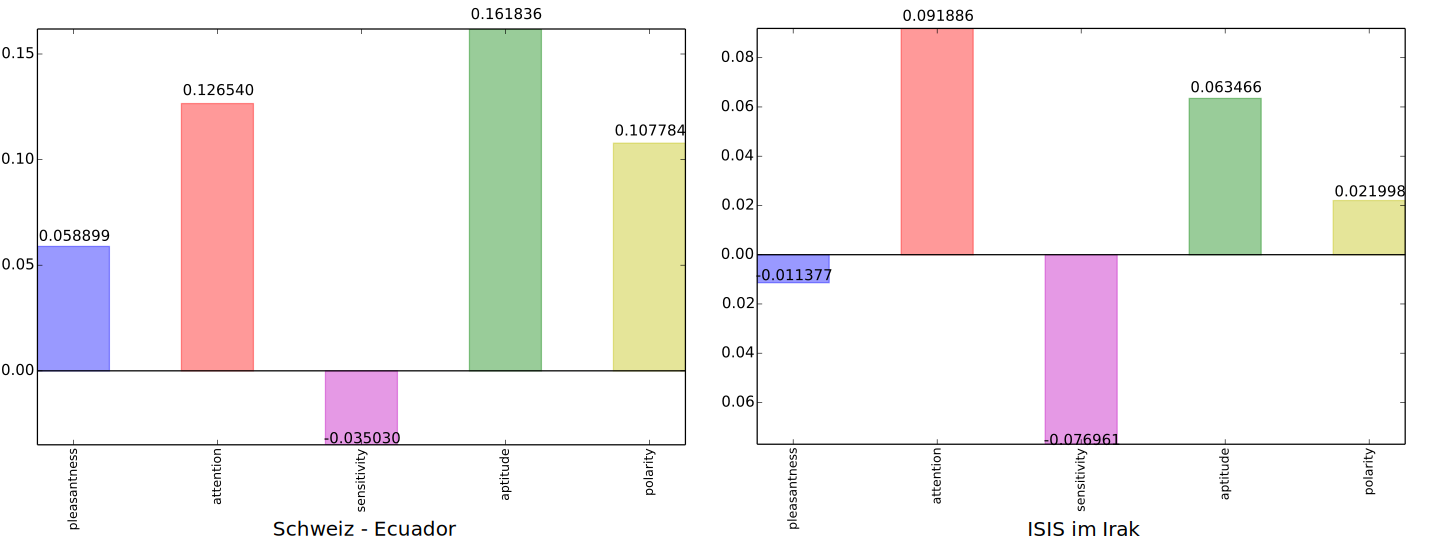
\includegraphics[width=0.8\textwidth]{images/schweizvsirak_senticnet.pdf}
  \caption[SenticNet: Schweiz - Ecuador vs. ISIS im Irak]{SASA: Schweiz - Ecuador vs. ISIS im Irak}
  \label{fig:senticnetanalysis}
\end{figure}

Die SASA Library (vgl. Abbildung \ref{fig:sasaanalysis}) hat viele der Irak-Tweets als neutral gelabelt. Dies würde sich mit meiner Beobachtung der vielen Zeitungsüberschriften decken. Weiter scheint der Algorithmus Probleme mit den sehr kurzen Tweets im Stil von \flqq \#Switzerland beats \#ecuador 2-1 at World \#EnnerValencia \#WorldCups\frqq zu haben. Er Kategorisiert diese gar nicht erst. 

Der SenticNet (vgl. Abbildung \ref{fig:senticnetanalysis}) Algorithmus zeigt für die Schweiz-Ecuador Tweets deutlich positivere Resultate als für die Tweets zum Treiben der ISIS Jihadisten im Irak. Diese Resultate scheinen plausibel zu sein.

\begin{figure}[h]
  \centering
  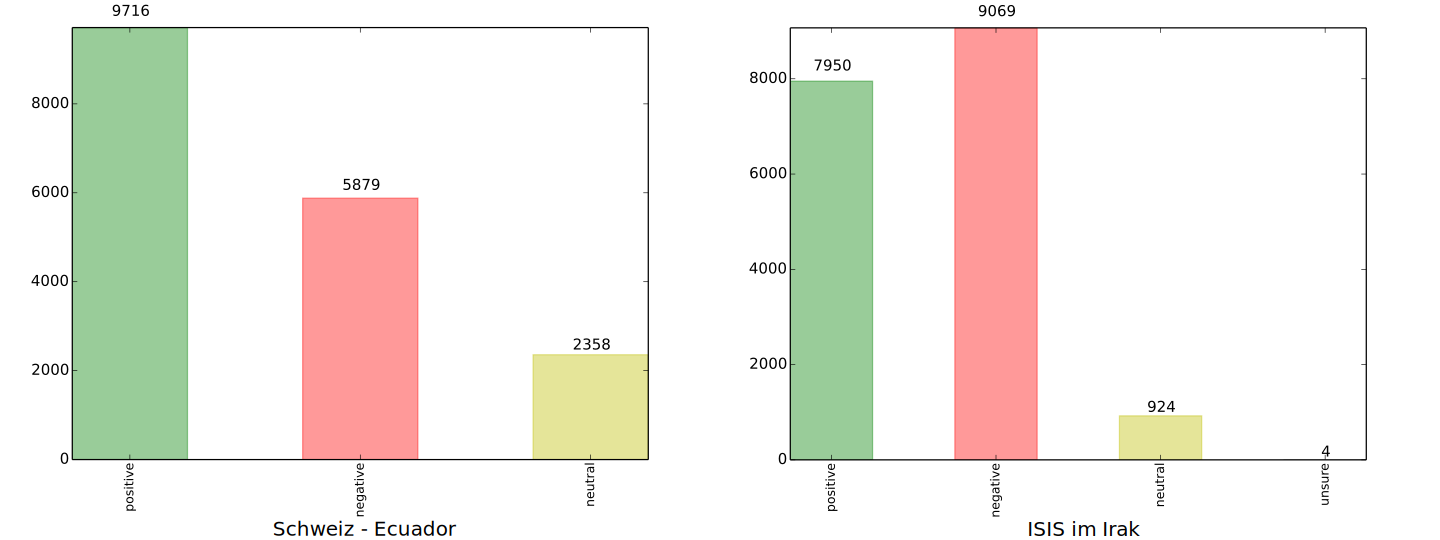
\includegraphics[width=0.8\textwidth]{images/schweizvsirak_sentiwordnet.pdf}
  \caption[SentiWordNet: Schweiz - Ecuador vs. ISIS im Irak]{SentiWordNet: Schweiz - Ecuador vs. ISIS im Irak}
  \label{fig:sentiwordnet}
\end{figure}

Auch die Resultate des SentiWordNet (Abbildung \ref{fig:sentiwordnet}) scheinen plausibel zu sein. Hier werden negative Emotionen aus den ISIS Tweets herausgelesen und das Schweizer Tor in der 93. Minuten wird zwar von der Mehrheit, jedoch nicht von allen Twitterern positiv beschrieben.

Diese Beobachtungen decken sich mit den Erkenntnissen von Pollyanna Gonçalves et al. \cite{comparing}. Um wirklich etwas darüber auszusagen müsste gefilterte, bereinigte und manuell klassifizierte Tweets zu unterschiedlichen Themen untersuchen.

\clearpage
\subsection{Parallelisierung}
Die Vorteile der Parallelisierung auf meinem 4-Kerne System waren bereits ab wenigen tausend Tweets spürbar. Um zu sehen wie viel die Parallelisierung wirklich aus macht, wurden die Tweets über die ISIS Jihadisten mehrfach mit unterschiedlicher Anzahl Prozesse vom Programm analysiert. Dabei sind mir vor allem Unterschiede in den Zeiten für die Analysen an sich (der parallelisierte Teil) und der Initialisierung ins Auge gefallen. 

\begin{figure}[h]
  \centering
  \includegraphics[width=0.8\textwidth]{images/parallelisierung_chart.png}
  \caption[Laufzeitverhalten bei unterschiedlicher Anzahl Prozesse]{Laufzeitverhalten bei unterschiedlicher Anzahl Prozesse}
  \label{fig:analyseparallel}
\end{figure}


In der Abbildung \ref{fig:analyseparallel} ist ersichtlich, wie die Zeit für die Initialisierung bis zum erreichen der physisch vorhandenen 4-Kerne praktisch konstant bleibt. Wenn man die Anzahl Prozesse weiter erhöht, nimmt die Dauer für die Initialisierung stark zu. Dies liegt daran, dass sowohl der SASA Algorithmus als auch der NLTK Classifier für jeden Prozess initialisiert werden müssen. Diese Initialisierungen sind sehr aufwändig und wenn die physisch vorhandenen 4-Kerne diese Aufgabe für mehr als 4 Prozesse erledigen sollen, dauert dies entsprechend länger.

Die Zeit für die Analyse ist bei einem Prozess am höchsten, und nimmt bis zum erreichen der 4 vorhandenen Cores um fast $\frac{2}{3}$ von 30s auf unter 10s ab. Wenn mehr Prozesse verwendet werden, wird diese Zeit nicht merklich erhöht aber sie nimmt auch nicht mehr ab.

Daraus lässt sich schlussfolgern, dass in dem gegebenen Setup 4 Prozesse die beste Performance bieten. Weiter könnte man daraus ableiten, dass die optimale Anzahl Prozesse der Anzahl verfügbarer Cores entspricht. Diese These könnte unter gleichen Testbedingungen auf verschiedenen Setups weiter untersucht und gegebenenfalls verifiziert oder falsifiziert werden. Die Einstellung zur Anzahl Prozesse kann im \lstinline$starter.py$ angepasst werden.
\clearpage
\section{Fazit}
Trotz anfänglichen Schwierigkeiten (Twitter API bietet keine Zeitraumsuche, keine Antwort vom SentiStrength Team) ist es gelungen einige Algorithmen zur Erkennung von Emotionen in Texten einzubinden. Es konnten sowohl Unterschiede zwischen den Resultaten der verschiedenen Algorithmen als auch die Performance Vorteile der Parallelisierung mit MPI aufgezeigt werden. Die Bewertung der Unterschiede der verschiedenen Algorithmen oder die Bewertung der Eignung der Algorithmen zum Erkennen von Emotionen in Tweets, würden einen Umfangreichen Datenkorpus mit gelabelten Tweets zu verschiedensten Themengebieten erfordern, war nicht Teil dieser Arbeit und könnte in weiteren Studien untersucht werden.

Durch äussere Umstände konnte das Projekt nicht komplett entsprechend der Anfänglichen Planung (Siehe Kapitel \ref{subsec:planung}) abgewickelt werden. Viele Termine wurden verschoben was dazu geführt hat, dass weniger Zeit im \flqq Reserveblock\frqq Endkorrektur und Abschluss zu Verfügung stand. Trotz diesen kleinen Terminverschiebungen, konnte sowohl das Produkt zum Analysieren von Twittermeldungen als auch die hier vorliegende Dokumentation im Zeitrahmen abgeschlossen werden. 

\clearpage

%%%
%%% end main document
%%%
%%%%%%%%%%%%%%%%%%%%%%%%%%%%%%%%%%%%%%%%%%%%%%%%%%%%%%%%%%%%%%%%%%%%%%%%%%%%%%%%

 \appendix  %% include it, if something (bibliography, index, ...) follows below
\begin{appendix}
%\input{content/99_anhang/anhang.tex}
\printglossary[title=Glossar]
%%% start a new page and display the list of figures
% \newpage
 \listoffigures

%%% start a new page and display the list of tables
% \newpage
 \listoftables

\lstlistoflistings


%%%%%%%%%%%%%%%%%%%%%%%%%%%%%%%%%%%%%%%%%%%%%%%%%%%%%%%%%%%%%%%%%%%%%%%%%%%%%%%%
%%%
%%% bibliography
%%%
%%% available styles: abbrv, acm, alpha, apalike, ieeetr, plain, siam, unsrt
%%%
 \bibliographystyle{plain}

%%% name of the bibliography file
 \bibliography{projekt.bib}

\end{appendix}
\end{document}
%%% }}}
%%% END OF FILE
%%%%%%%%%%%%%%%%%%%%%%%%%%%%%%%%%%%%%%%%%%%%%%%%%%%%%%%%%%%%%%%%%%%%%%%%%%%%%%%%
%% Local Variables:
%% mode: outline-minor
%% OPToutline-regexp: "%% .*"
%% OPTeval: (hide-body)
%% emerge-set-combine-versions-template: "%a\n%b\n"
%% End:
%% vim:foldmethod=marker
